%! root=./main.tex
\section{Provably Safe CFI Implementation}

We have implemented a CFI rewriter in Gallina using the aforementioned case-analytical structure.
The rewriter accepts an ARMv7 binary program and a control-flow policy as input and produces a rewritten binary with IRMs that enforce the policy.
Furthermore, we have proved the implementation to be correct using the proof structure outlined above.
The result is an extractable OCaml program with machine-checked correctness guarantees.

\subsection{Rewriter Architecture}

Our rewriter operates by analyzing each instruction in the input program and dispatching to specialized rewriting functions based on the four cases identified earlier.
The overall architecture follows a compositional design where each component handles one category of instruction sequences and produces provably-safe inline reference monitors.

\paragraph{Safe Instructions} are those that do not affect control flow: arithmetic operations, memory loads and stores to non-executable regions, and other data processing instructions.
These instructions require no rewriting for CFI enforcement, as they cannot violate the control-flow policy.
However, they must still be relocated to account for the insertion of IRMs elsewhere in the program.
Our rewriter preserves these instructions unchanged but updates any PC-relative addressing to reflect their new locations.

\paragraph{Static Branches} (i.e., direct jumps and calls with compile-time constant targets) are inherently policy-compliant if their target is valid according to the CFI policy.
The challenge is that IRM insertion causes code relocation, invalidating original branch targets.
Our rewriter handles static branches by computing new target addresses that account for the cumulative size of all IRMs inserted before the target location.
The rewritten instruction uses the updated immediate offset to reach the intended destination.

For conditional branches, we preserve the original condition code while updating only the target offset.
This ensures that the dynamic control flow behavior matches the original program while satisfying the CFI policy.

\paragraph{Dynamic Branches} (e.g., indirect jumps, returns, and jump tables) pose the primary challenge for CFI enforcement, as their targets are computed at runtime.
Our rewriter instruments these instructions with table-lookup IRMs that validate destinations before transferring control.

\paragraph{Invalid instructions} in the original binary could potentially be exploited to bypass CFI checks.
Our rewriter replaces any invalid or unpredictable instruction sequences with unconditional branches to a designated abort routine.
The abort routine terminates execution safely, preventing any policy violations.

\subsubsection{Hash-Based Table Lookup.}

Unlike traditional CFI implementations that use linear arrays indexed directly by target address, our approach uses a compact hash table indexed by a hash of the target address.
For each dynamic branch site, the rewriter:

\begin{enumerate}
    \item Computes an optimal hash function of the form $H(x) = (x \ll sl) \gg sr$, where $sl$ and $sr$ are shift parameters chosen to prevent collisions among the policy-permitted destinations for this branch site.
    \item Generates a lookup table where $\mathit{table}[H(d)] = d'$ and $\mathit{table}[H(d')] = d'$ for each permitted destination $d$ (mapped to its new location $d'$).
    \item Inserts validation code that computes $H(\mathit{target})$, looks up the result in the table, and transfers control to the retrieved address, which is either permitted by the policy or the abort address.
\end{enumerate}

\begin{figure}
    \centering
    % drawio file link:
    % https://drive.google.com/file/d/1BRexH1KjlPXB-1lNX2qnoN52LuUoykd4/view
    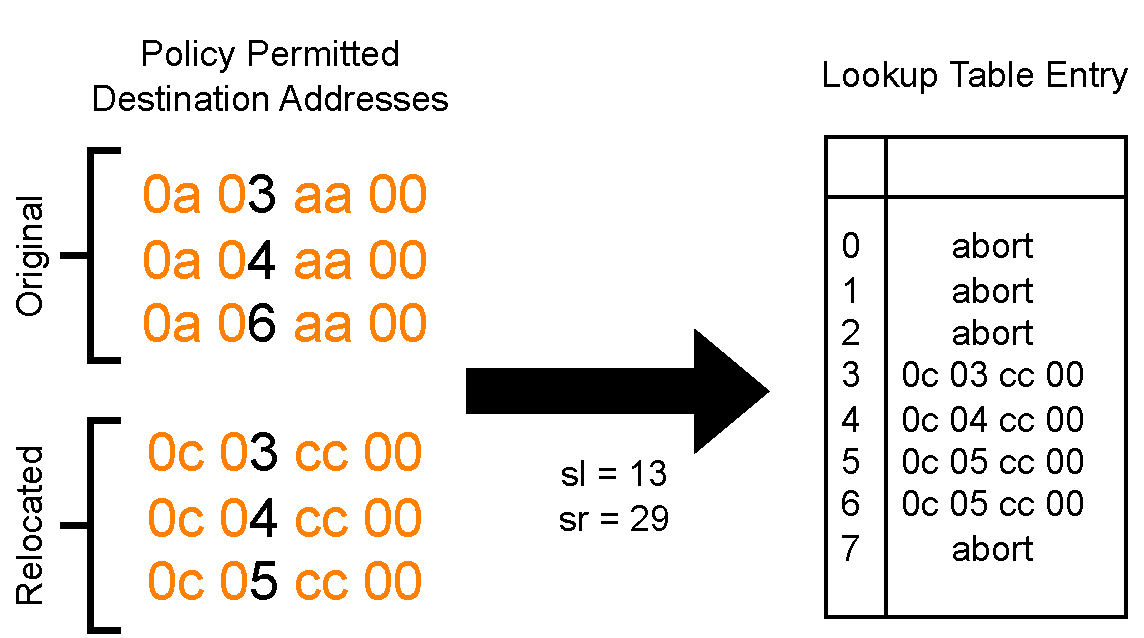
\includegraphics[width=1.0\columnwidth]{figs/CFI_hashtable.drawio.pdf}
    \vspace{-10pt}
    \caption{Example Hash Table Entry}
    \label{fig:cfi_hash_table}
\end{figure}

\subsection{Proof Architecture}

\begin{equation}\label{eq:cfi_safety}
\begin{aligned}
& \forall\ \ \mathit{pol}, \mathit{code}, \mathit{irms}, \mathit{tables}, s_0, t, \\
&\ \quad \texttt{cfi\_rw}(\mathit{pol}, \mathit{code}) = \texttt{Some} (\mathit{code'}, \mathit{tables})\ \land \\
&\ \quad \mathit{valid}(\mathit{abort\_index})\ \land\\
&\ \quad \mathit{store\_invs}(s_0) \implies \\
&\quad \mathit{satisfies\_all}(\mathit{code'}, \mathit{cfi\_invs}, \mathit{cfi\_exits}, t)
\end{aligned}
\end{equation}

% If you start at an IRM, you will either
% - end up at another IRM (and therefore stay in the policy)
%   with correct flags
% - leave the bounds of the rewritten code (e.g. to interface with the operating system), at which point all security guarantees are lost
% - raise an exception

% discuss these assumptions, impliciations of the conclusion, etc.

Equation~\ref{eq:cfi_safety} presents our main safety theorem, which states that any execution trace starting at the entrypoint of code produced by \texttt{cfi\_rw} will satisfy all CFI invariants.
Each invariant states that at the beginning of each IRM block, either
\begin{enumerate}
    \item control will always reach a CFI invariant point and satisfy the safety guarantee placed there,
    \item control will leave the bounds of the rewritten code (e.g. to interface with the operating system), at which point no security guarantee is provided, or
    \item a hardware exception is raised.
\end{enumerate}

% \subsection{Architecture}

% Because you started at an IRM, you know that the code came out of the rewriter
% If it came out of the rewriter, then one of the rewriter components generated the IRM
% So, do case analysis on which component generated the IRM and show that each component only generates code that meets the above specification

% These cases look like one of
% 1. Block is all safe instructions, so just run them all and fall through (easy)
% 2. Dynamic jump occurs, so we need to do a table lookup and then jump to a valid address (hard)
% 3. Block contains invalid instructions, so replace them with aborts

% Might want to just get rid of the section split
\subsection{Supporting Safety Lemmas}

The main safety theorem is proved through a hierarchy of supporting lemmas that establish safety properties for each IRM category.
These lemmas follow a common structure: they take the rewriter output for a specific instruction, assume the initial store is well-formed, and prove that execution satisfies the permitted step relation and reaches the next CFI invariant point.
Well-formed stores must have the IRM code and lookup tables at the correct location in memory, and these regions must be marked non-writable.

\subsubsection{Static Jumps and Safe Instructions.}

% Cases 1,2 above
For safe instructions, we prove a \emph{fallthrough lemma} establishing that execution proceeds to the next instruction while preserving all invariants.
The key insight is that safe instructions cannot modify control flow.

Safe instructions are characterized by (1) never leading to an exit point, and (2) maintaining critical processor flags such as endianness and instruction set.
Individual lemmas establish that common instructions (e.g., loads, stores, arithmetic operations, and bit manipulations) satisfy this predicate by analyzing their PIL semantics.

For static branches, the proof must relate the original branch target to its relocated counterpart.
We define address mapping functions $i2i'$ and $i'2i$ that convert between original and relocated addresses.
The key lemma shows that executing a rewritten static branch transfers control to an address $a'$ such that either $a' = a_\mathrm{abort}$, or the original block index $i'2i(\frac{a'}{4})$ is policy-permitted from the source block.

An important subtlety is handling conditional branches.
The rewriter wraps conditional IRMs with a branch that skips the IRM body when the condition is false.
The proof uses case analysis on the condition evaluation: if false, execution falls through to the next block; if true, the IRM executes and the nested lemma applies.

\subsubsection{Dynamic Jumps.}

% Case 3 above

Dynamic jump safety requires a multi-stage proof corresponding to the hash table construction and lookup process.

We first prove that the hash parameter search produces collision-free functions.
The rewriter searches for shift parameters $(sl, sr)$ such that applying $H(x) = (x \ll sl) \gg sr$ to all policy-permitted destinations produces distinct values, with at most one collision between an original destination $d$ and its relocated counterpart $d'$.
This collision tolerance is essential because runtime register values might contain either the original or relocated address depending on execution history.

Given valid hash parameters, we prove that the generated table maps each hash value to a safe destination.
The proof proceeds by induction on the policy's destination list, showing that each table entry is either the abort address or a relocated destination corresponding to a policy-permitted original address.
This requires establishing a predicate for \emph{safe exits}: an address $a$ is safe from source block $i$ if either $a = a_\mathrm{abort}$, or there exists an original destination $d$ such that $i2i'(d) = a$ and $d \in \mathit{pol}(i)$.

The table lookup sequence consists of hash computation, address scaling, table base addition, and load.
The composition of these steps shows that the final loaded jump target satisfies the safe exit predicate.

\subsubsection{Invalid Instructions.}

% Case 4 above
Invalid or unpredictable instructions are replaced with unconditional branches to the abort routine.
The proof is straightforward: we symbolically execute the generated instruction and show that it unconditionally transfers control to $a_{\text{abort}}$, which trivially satisfies the permitted step relation.

All potential invalid instructions are provably caught by this verified replacement.
The rewriter explicitly handles all known instructions, and replaces all unknown instructions with jumps to the abort routine.

\subsubsection{Proof Composition}

The final safety theorem composes these category-specific lemmas through a master case analysis lemma that examines the rewriter's output for each instruction.
Given the rewriter's output for instruction at index $i$, the lemma:

\begin{enumerate}
    \item Determines which category the instruction falls into based on the rewriter's behavior
    \item Retrieves the appropriate category lemma
    \item Applies the lemma to establish that execution from address $i'$ satisfies permitted steps and reaches the next invariant point at $i' + |\mathrm{irm}|$
\end{enumerate}

This structure enables modular reasoning: each category's safety is proved independently, and the composition is purely structural case analysis.
The proof of the main safety theorem then proceeds by induction on the execution trace, applying this per-instruction lemma at each IRM block boundary.

\subsection{Supporting Formalizations}

% CFI_nextinv
% SafeE, SafeP, SafeT
% cfi_step and related work on symbolically interpreting IL in hypotheses

% \subsubsection{Rewriter Interface}

% Takes as input
% - CFI Policy
% - Program as list of instructions
% - Location of old program address
% - Desired location of new program address
% - Desired location of lookup tables
% - Desired location of abort subroutine
% Returns OPTIONALLY
% - List of IRM blocks (sequences of instructions) to place at new program address
% - List of lookup tables to place at lookup table address
% - If inputs found to be malformed, returns None

\subsection{Construction of Secure Binary}

\todo{Do we need to discuss the python script that reconstructs the binaries?}

% Python script that objcopies (I think?) the new instructions and tables into the right locations in the original program. Max knows more about this than I do.

% \section{Technical}

% % A distillation of the SafeDest_rewrite_inst we are currently working on.
% % The original theorem is more complicated, stating that the trace may have a prefix
% % before the part that started in the block. This draft is simpler, instead stating that
% % the trace began at a block. Another difference is that this omits the hypotheses that the
% % table and block are maintained in memory as the IRM block is executed.
% %

% \begin{equation}\begin{aligned}
%     & \forall t\, tbl\, m\, \,i\, \,pol, \,\,rewrite\_inst\, i\, pol\, =\, (b,\,tbl) \\
%     & \land\: starts\_with\_memory \,\,t\,\,m  \\
%     & \land\: starts\_in\_block \,\,t\,\,b \\
%     & \land\: table\_in\_memory \,\,tbl\,\,m \\
%     & \land\: block\_in\_memory \,\,b\,\,m \\
%     & \implies safely\_exits\_block \,\,t\,\,b
% \end{aligned}\end{equation}

% The key theorem states that the rewriter's output is safe per rewritten instruction block.
% All traces that start at the beginning of a block exit to a safe destination.
% Safe destinations are either the start of a block corresponding to the policy-permitted instruction or the safety-abort address.

\subsection{Symbolic Execution of Quantified Programs}

Proving some instruction blocks are safe requires reasoning about their destination address and its relationship to the table returned by the rewriter.
The destination address is computed from the table through a sequence of instructions, and the proof requires reasoning about those instructions despite the absence of a concrete program to analyze.
It turns out that for symbolic execution, it is sufficient to know that the block is in the same memory address that the trace is executing from, exactly our assumptions.

% Steps for symbolic execution:

% \begin{enumerate}
%     \item prepXP - prepare the XP hypothesis to get it in normal form. Original hyp: \texttt{exec\_prog p (((Addr a', s') :: t1) ++ t0)}; new hyp: \texttt{exec\_prog p
%     ((Addr a', s') :: t ++ [(Addr (Z.to\_N (i2i' i) * 4 + 4 * 0), s1)])}
%     \item rireduceRI - reduce the rewriter output hypothesis to a concrete list of assembly instruction expressions, this note currently covers both rireduceRI and rireduceSplit.
%     \begin{itemize}
%         \item Original hyp: \texttt{  rewrite\_pc
%     (ARM\_data\_r op Z14 S (unused\_reg 15 15 15) (unused\_reg 15 15 15) imm5
%        type (unused\_reg 15 15 15)) (unused\_reg 15 15 15) tc
%     (pol i) i2i' cond i ti ai = Some (irm', table, tc')};
%         \item     new hyp: \texttt{  arm\_assemble\_all
%     [ARM\_B (invert\_cond cond) (Z.pos (Pos.of\_succ\_nat 13) - Z1);
%      STR (unused\_reg 15 15 15) SP Z\_4;
%      MOVW (unused\_reg 15 15 15) (Z.land (Z4 * i + Z8) Z0xffff);
%      MOVT (unused\_reg 15 15 15) (Z.land (Z.shiftr (Z4 * i + Z8) Z16) Z0xffff);
%      ARM\_data\_r op Z14 S (unused\_reg 15 15 15) (unused\_reg 15 15 15) imm5
%        type (unused\_reg 15 15 15);
%      UBFX (unused\_reg 15 15 15) (unused\_reg 15 15 15) (z2 - Z2) z0;
%      LSL (unused\_reg 15 15 15) (unused\_reg 15 15 15) Z2;
%      ARM\_data\_i ARM\_ADD Z14 0 (unused\_reg 15 15 15)
%        (unused\_reg 15 15 15)
%        (Z.lor (Z.shiftl Z4 Z8) (Z.land (Z.shiftr (Z4 * z1) Z24) Z0xff));
%      ARM\_data\_i ARM\_ADD Z14 0 (unused\_reg 15 15 15)
%        (unused\_reg 15 15 15)
%        (Z.lor (Z.shiftl Z8 Z8) (Z.land (Z.shiftr (Z4 * z1) Z16) Z0xff));
%      ARM\_data\_i ARM\_ADD Z14 0 (unused\_reg 15 15 15)
%        (unused\_reg 15 15 15)
%        (Z.lor (Z.shiftl Z12 Z8) (Z.land (Z.shiftr (Z4 * z1) Z8) Z0xff));
%      ARM\_data\_i ARM\_ADD Z14 0 (unused\_reg 15 15 15)
%        (unused\_reg 15 15 15) (Z.land (Z4 * z1) Z0xff);
%      LDR (unused\_reg 15 15 15) (unused\_reg 15 15 15) 0;
%      STR (unused\_reg 15 15 15) SP Z\_8; LDR (unused\_reg 15 15 15) SP Z\_4;
%      LDR PC SP Z\_8] = Some irm'}
%     \end{itemize}

%     \item calc\_irm'\_len - calculate the length of the block computed in the previous step, rirediceRI. This is used to prove contradictions and safety in certain proof cases.
%     \item eval\_first\_inst - Given the first instruction of a trace originating somewhere in the block, symbolically execute it. This prevents executing it twice - once for the case where the intervening trace is empty, once for the case where it is not. Does not take arguments, finds the correct hypothesis in context using some brittle assumptions.
%     \item XP\_cases - destructs the exec\_prog assumption based on whether the intervening trace is empty or not. Presently admits the simple case where it is empty, and we step directly to an instruction also in the block.
%     \item unify\_CS - unifies the instruction execution evaluated in eval\_first\_inst with the step assertions from case analysis in XP\_cases
%     \item reformat\_XP - reformats the exec\_prog trace to be in the \texttt{4 * index} format eval\_first\_inst expects.
%     \item solve\_cond\_skip - solves the case where the block of a conditional instruction is skipped over and the trace keeps going.
% \end{enumerate}